\chapter{مقدمه}
\section{مقدمه}
رایانش ابری\LTRfootnote{Cloud Computing} یکی از حوزه‌های در حال تحول کامپیوتر است که به یک جنبه‌ی حیاتی از فناوری و مشاغل مدرن تبدیل شده است. این الگو همچون انقلابی، شیوه‌ی ارائه و مصرف منابع محاسباتی را متحول کرده است و فرصت‌های جدیدی را برای سازمان‌ها فراهم کرده تا کارایی و رقابت خود را بهبود بخشند. یکی از پایه‌ای‌ترین و رایج‌ترین شکل‌های رایانش ابری، زیرساخت به عنوان خدمت (\lr{IaaS})\LTRfootnote{Infrastructure As A Service} است که منابع محاسباتی مجازی مانند فضای ذخیره‌سازی، قدرت پردازش و پهنای باند را از طریق اینترنت در اختیار کاربران قرار می‌دهد.\cite{Mell_2011}

\begin{figure}[h]
	\vspace{1cm}
	\centering
	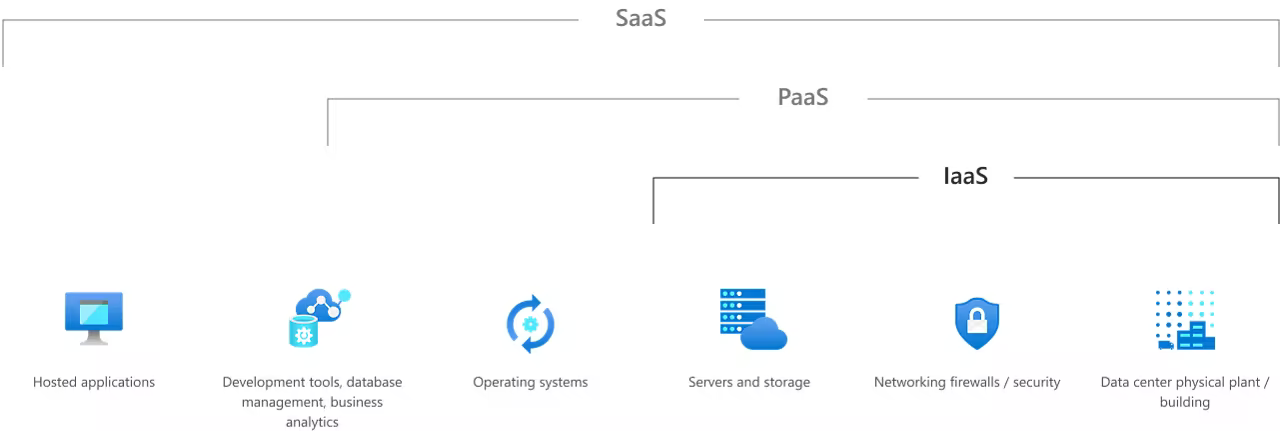
\includegraphics[scale=0.35]{figures/cloud_computing_models.png}
	\caption{انواع مدل‌های رایانش ابری\cite{microsoft_cc_models}}
	\label{fig:cc_models}
\end{figure}

این الگو را از دو دیدگاه می‌توان بررسی کرد. دیدگاه اول مختص کاربران مصرف‌کننده است که برای استفاده و مصرف منابع دیگر دغدغه‌ای نسبت به زیرساخت استفاده شده برای ارائه‌ی خدمات ندارند. دیدگاه دوم مربوط به ارائه دهندگان این خدمت است. از این دیدگاه، توسعه یک سکو\LTRfootnote{Platform} کارآمد و قابل اعتماد که بتواند مشتریان را جذب و حفظ کند، بسیار مهم است. از این رو، شرکت‌ها و توسعه‌دهندگان سراسر دنیا همواره سعی در توسعه و فراهم‌کردن ابزارها با این هدف دارند. یکی از معروف‌ترین این شرکت‌ها، شرکت \lr{VMWare} است که برنامه‌های فراوانی برای فراهم کردن زیرساخت ارائه‌ی خدمات ابری توسعه داده است. چالش بعدی ارائه‌دهندگان، فراهم کردن و طراحی یک رابط برنامه‌نویسی (\lr{API})\LTRfootnote{Application Programming Interface} است که بتواند با مشتریان و ارائه دهنده زیرساخ\LTRfootnote{Infrastructure Provider} تعامل داشته باشد و آن‌ها را قادر سازد منابع مجازی خود را مدیریت کنند.
\section{تعریف مسئله}
در این پروژه قصد داریم که خدمات جامع یک ارائه‌دهنده‌ی زیرساخت به عنوان خدمت را که بر بستر ابزار \LTRfootnote{https://vmware.com/products/cloud-director.html}\lr{VMWare Cloud Director} فراهم شده است را توسط یک رابط برنامه‌نویسی به کاربران ارائه دهیم. برای این هدف، باید خدمات کاربردی، مدیریتی، نظارتی و امنیتی را در یک لایه‌ی جدا تعریف کنیم و این لایه از برنامه‌ی خود را با ابزار زیرساختی در تعامل نگه داریم. 
\section{راه حل پیشنهادی}
برای توسعه این محصول، بایستی در ابتدا با بررسی نیازمندی‌ها و محدودیت‌های زیرساخت و کاربران، اقدام به طراحی کلی سامانه کرد. با توجه به گسترده بودن این نیازمندی‌ها و توسعه‌پذیری جداگانه آن‌ها، باید طراحی کلی این سامانه به صورت پیمانه‌ای\LTRfootnote{Modular}و با کمترین وابستگی میان واحد‌ها باشد. در این گزارش ابتدا به طراحی و شرح قسمت‌های مختلف سامانه می‌پردازیم و سپس جزئیات فنی هر قسمت و تعامل قسمت‌ها را بررسی می‌کنیم.
\section{نیازمندی‌های پروژه}
همانطور که قبلا پرداخته شد، جهت ارائه‌ی این خدمات، نیازمند نصب و اجرای ابزار \lr{VMWare Cloud Director} داریم. این ابزار جهت اجرا، نیازمند منابع اختصاصی ذخیره‌سازی، پردازشی و شبکه‌ای است که باید پیش از اجرا فراهم گردد. همچنین اجرای سامانه‌ی رابط برنامه‌نویسی، نیازمند چندین ماشین مجازی و  ترجیحا یک محیط سکو به عنوان خدمت همانند کوبرنتیز\LTRfootnote{Kubernetes} است.
